\documentclass[main.tex]{subfiles}
\begin{document}

\href{https://www2.seas.gwu.edu/~simhaweb/quantum/modules/module8/module8.html}{Module 8: Quantum circuits - reversible construction}\\

\begin{enumerate}

\item[] \textbf{In-Class Exercise 1:} \textbf{Q} Write out the AND-with-$X$ and OR-with-$X$ tables. Are these gates reversible? 
    \textbf{A} Neither the Table \ref{tab:AndX} gate or Table \ref{tab:OrX} gate is reversible because both contain outputs that cannot be used to uniquely determine their inputs.
    \begin{table}
    \centering
    \begin{tabular}{ |c|c|c|c| } 
     \hline
     \multicolumn{2}{|c|}{Inputs} & \multicolumn{2}{c|}{Outputs} \\ 
     \hline
     x & y & x & x $\wedge$ y \\ 
     \hline
     0 & 0 & 0 & 0 \\ 
     \hline
     0 & 1 & 0 & 0 \\ 
     \hline
     1 & 0 & 1 & 0 \\ 
     \hline
     1 & 1 & 1 & 1 \\ 
     \hline
    \end{tabular}
    \caption{AND-with-X}
    \label{tab:AndX}
    \end{table}
    
    \begin{table}
    \centering
    \begin{tabular}{ |c|c|c|c| } 
     \hline
     \multicolumn{2}{|c|}{Inputs} & \multicolumn{2}{c|}{Outputs} \\ 
     \hline
     x & y & x & x $\vee$ y \\ 
     \hline
     0 & 0 & 0 & 0 \\ 
     \hline
     0 & 1 & 0 & 1 \\ 
     \hline
     1 & 0 & 1 & 1 \\ 
     \hline
     1 & 1 & 1 & 1 \\ 
     \hline
    \end{tabular}
    \caption{OR-with-X}
    \label{tab:OrX}
    \end{table}

\item[] \textbf{In-Class Exercise 2:} \textbf{Q.} Show how the Fredkin gate can implement the classical AND and OR gates. 
    \textbf{A.} We can write the Fredkin algebraically on standard-basis vectors as 
    \begin{align*}
        F|x, y, z\rangle & = \left|x, x^{\prime} y+x z, x^{\prime} z+x y\right\rangle
    \end{align*}
    where $x, y, z$ are all binary variables. Figure \ref{fig:FredkinAND} implements a classical AND gate and Figure \ref{fig:FredkinOR} implements a classical OR gate. 

    \begin{figure}
        \centering
        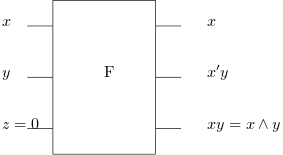
\includegraphics[width=3in]{modules/figs/m08/FredkinAnd.png}
        \caption{Fredkin classical AND}
        \label{fig:FredkinAND}
    \end{figure}

    \begin{figure}
        \centering
        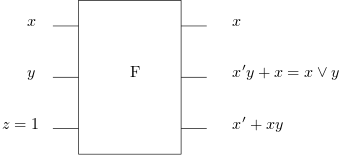
\includegraphics[width=3in]{modules/figs/m08/FredkinOr.png}
        \caption{Fredkin classical OR}
        \label{fig:FredkinOR}
    \end{figure}

\item[] \textbf{In-Class Exercise 3:} \textbf{Q.} Verify that the above circuit does indeed represent the functionality of a full adder. \textbf{A.}

\item[] \textbf{In-Class Exercise 4:} \textbf{Q.} Use the above approach to derive the outer-product form and matrix for the unitary version of a classical OR gate. \textbf{A.}

\end{enumerate}
\end{document}